\subsection{Spettrometria $\gamma$}
Riassumiamo il principio di misura dell'energia del nostro spettrometro:
\begin{itemize}
	\item particelle cariche attraversano il cristallo scintillatore rilasciando energia all'interno per eccitazione/ionizzazione degli elettroni dello stesso;
	\item lo scintillatore produce luce in funzione dell'energia rilasciata ($\sim \SI{40}{fotoni \; keV^{-1}}$ nel NaI(Tl));
	\item i fotoni raggiungono il fotomoltiplicatore dopo essere stati riflessi sulle pareti del cristallo (rivestite di materiale riflettente) e nella guida ottica;
	\item il fotomoltiplicatore amplifica il segnale dei fotoni e produce in uscita un segnale (negativo e di breve durata: $\sim \SI{10}{\nano s}$) di picco proporzionale al numero di fotoni;
	\item la base del fotomoltiplicatore in dotazione fornisce anche un segnale pre-amplificato positivo a bassa impedenza (perciò di lunga durata $\sim \SI{1}{\micro s}$);
	\item questo segnale viene riconosciuto dal formatore/amplificatore che produce in uscita un segnale gaussiano di durata nota ($\SI{10}{\micro s}$) e di picco proporzionale all'energia rilasciata;
	\item l'output dell'amplificatore va all'ADC (tipicamente triggerato da un segnale esterno) che campiona sul massimo del segnale in una finestra temporale imposta dal trigger e converte il segnale in tensione in un segnale digitale a 13 bit.
\end{itemize}
Ciascuno di questi processi sarà caratterizzato da una:
\begin{itemize}
	\item\emph{funzione di risposta}: la funzione che da un certo input mi dà l'output medio (ad esempio energia della particella vs energia media rilasciata, energia rilasciata vs numero medio di fotoni prodotti, segnale in tensione vs digit, tutte in prima approssimazione lineari nel nostro range di lavoro\footnote{discuteremo nel seguito la validità di questa approssimazione});
    \item una \emph{distribuzione di risposta}: la distribuzione degli output a input fissato (ad esempio la distribuzione dei fotoni prodotti ad una energia fissata, queste ci aspettiamo avranno generalmente un forma a campana, in prima approssimazione gaussiana).
\end{itemize}
La misura finale avrà per funzione di risposta la composizione di tutte queste funzioni di risposta e per distribuzione di risposta la convoluzione delle distribuzioni di risposta (quest'ultima determinerà la risoluzione sperimentale).

Nella nostra esperienza lo spettrometro dovrà misurare l'energia di fotoni $\gamma$ che, essendo neutri, devono prima interagire con la materia del rivelatore e trasferire tutta o parte della loro energia a particelle cariche, delle quali sarà poi misurabile l'energia nel modo descritto sopra. Bisogna quindi analizzare le interazioni fotone-materia per modelizzare gli spettri che andremo poi ad osservare.

%%%%%%%%%%%%%%%%%%%%%%%%%%%%%%%%%%%%%%%%%%%%%%%%%%%%%%%%%%%%%%%%%%%%%%%%%%%%%%%%%%%%

\subsubsection{Interazione fotone-materia}
I principali meccanismi di interazione dei fotoni con la materia sono:
\begin{itemize}
	\item assorbimento fotoelettrico;
	\item scattering Rayleigh;
	\item scattering Compton;
	\item produzione di coppie.
\end{itemize}
  
 \paragraph{Assorbimento fotoelettrico}
 Il fotone incidente è completamente assorbito e ionizza l'atomo, ovvero estrae un elettrone di energia cinetica $T_e = E_{\gamma} - E_b$, dove $E_{\gamma}$ è l'energia del fotone incidente e $E_b$ è l'energia di legame, solitamente piccola se paragonata a $E_{\gamma}$. Nel nostro caso l'energia di legame vale al massimo $\sim \SI{33}{keV}$ per gli elettroni 1s dello iodio, da confrontarsi con l'energia dei fotoni $\gamma$ del \co\;: \SI{1.17}{MeV} e \SI{1.33}{MeV}. Il risultato finale è una particella carica nello scintillatore con approssimativamente la stessa energia del fotone incidente.
 Un elettrone con energia cinetica di $\SI{1}{MeV}$ ha un range in NaI di $\sim \SI{2}{mm}$ FONTE CIPPA LIPPA, questo vuol dire che questi fotoni perdono tutta la loro energia nel nostro rivelatore (un cilindro retto $\sim \SI{5}{cm} \times \SI{5}{cm}$). 

 \paragraph{Scattering Rayleigh}
 Nello scattering Rayleigh l'intero atomo funge da bersaglio, perciò dopo l'urto il fotone cambia direzione e l'atomo rincula per conservare il momento. Data la grande massa dell'atomo (rispetto all'energia del fotone) l'energia scambiata è trascurabile e il fotone uscente ha praticamente la stessa energia iniziale. \`E chiaro quindi che i fotoni non potranno essere rivelati in uno scintillatore con questo meccanismo perché nessuna energia viene rilasciata all'interno.
 
 \paragraph{Scattering Compton}
 Se il fotone è abbastanza energetico può urtare un singolo elettrone. Per fotoni di questo tipo l'energia di legame può essere in prima approssimazione trascurata e si può trattare l'elettrone come libero. Nello stato finale troviamo il fotone che è stato deviato di un certo angolo $\theta$ rispetto alla sua direzione iniziale e ha ceduto parte della sua energia all'elettrone. La relazione tra energia del fotone dopo lo scattering e angolo è:
 \begin{equation}
 \label{energia_compton}
 E' = \frac{E}{1+\frac{E}{m_ec^2}(1-\cos(\theta))}   
 \end{equation}
 Quello che misureremo nello spettroscopio sarà l'energia ceduta all'elettrone cioè $E-E'$. Quando un fotone fa scattering Compton nel nostro spettroscopio non abbiamo modo di conoscere l'angolo di scattering e non è possibile da una singola misura ricavare l'energia del fotone incidente.
 La sezione d'urto differenziale di questo processo (anche nota come formula di Klein–Nishina) è:
 \begin{equation}
 \label{klein-nishina}
 \frac{d\sigma}{d\cos(\theta)} = \frac{\pi}{m_e^2} \cdot\left(\frac{E'}{E}\right)^2 \cdot \left(\frac{E}{E'} + \frac{E'}{E} - \sin^2(\theta)\right)
 \end{equation}
 dove $\frac{E'}{E}$ contiene implicitamente l'angolo: $\frac{E'}{E} = \frac{1}{E(1-\cos(\theta))/(m_ec)}$
 La sezione d'urto differenziale è graficata in \autoref{fig:klein-nishina} ed è da qui evidente come all'energia di $\sim \SI{1}{MeV}$ è molto più probabile che il fotone sia deviato poco.
 
 \begin{figure}[h]
 	\centering
 	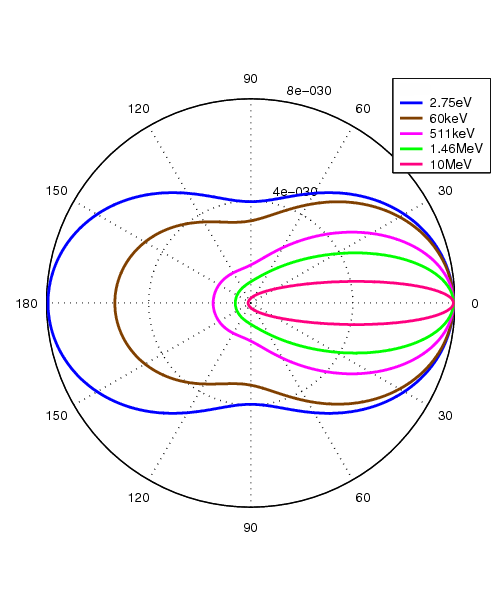
\includegraphics[width=16em]{klein-nishina}
 	\caption{\label{fig:klein-nishina}Sezione d'urto in funzione dell'angolo di scattering Compton}
 \end{figure}

 \paragraph{Produzione di coppie}
 Il fotone $\gamma$ può fare scattering con un fotone del campo e.m. del nucleo (o meno probabilmente di un elettrone) e produrre una coppia $e^+e^-$. Aaffinchè questo processo sia accessibile cinematicamente l'energia del fotone deve essere $> \SI{1.02}{MeV}$, quindi questo processo è possibile per i fotoni del \co\;  e del \na, tuttavia come vederemo questo processo è largamente trascurabile a queste energie, rispetto agli altri in gioco.
 
 %%%%%%%%%%%%%%%%%%%%%%%%%%%%%%%%%%%%%%%%%%%%%%%%%%%%%%%%%%%%%%%%%%%%%%
 
 \subsubsection{Sezione d'urto fotone-materia}
 La sezione d'urto fotone-materia per ciascuno dei processi prima descritti dipenderà dallo Z del materiale. In generale a basse energie ($ < \SI{10}{keV}$) sarà dominante l'assorbimento fotoelettrico, ad alte energie ($>\SI{100}{MeV}$) predominerà la produzione di coppie mentre lo scattering Compton sarà dominante in un range intermedio. L'estensione di questo range è maggiore al diminuire di Z come è chiaro dalla \autoref{fig:photon_cross_section_pdg}.
 
  \begin{figure}[h]
 	\centering
 	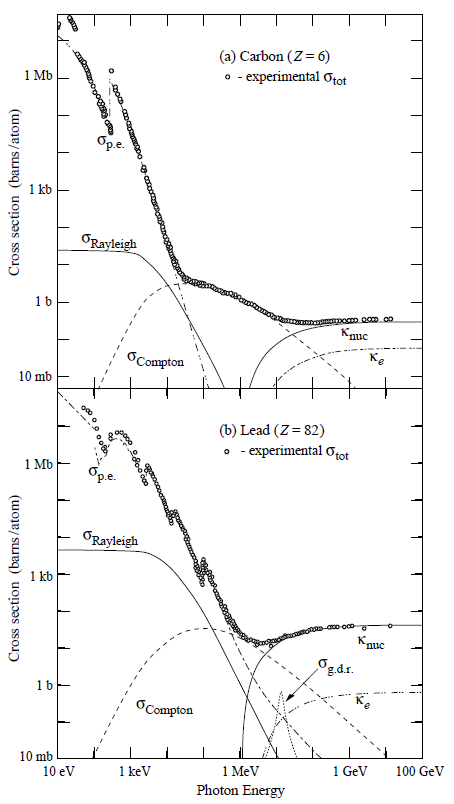
\includegraphics[width=16em]{cross_section_photon_pdg}
 	\caption{\label{fig:photon_cross_section_pdg}Sezione d'urto in funzione dell'energia per i vari processi nel carbonio e nel piombo FONTE CIPPLIPPA}
 \end{figure}

 \paragraph{Scelta del materiale per bersaglio e spettrometro}
 Nella nostra esperienza il bersaglio sarà di carbonio, mentre lo spettrometro è un cristallo di NaI ($\text{Z}(\text{Na})=11$, $\text{Z}(\text{I})=53$). Questa scelta è giustificata dal fatto che nel carbonio, all'energia dei fotoni del \co\; la sezione d'urto dell'assorbimento fotoelettrico è ampiamente trascurabile e l'energia del fotone è più facilmente misurabile dai fotopicchi associati all'assorbimento fotoelettrico. Sarà perciò preferibile usare il cristallo di NaI come spettrometro poichè a $\sim{1}{MeV}$ il rapporto tra sezione d'urto Compton e sezione d'urto dell'assorbimento fotoelettrico vale $\sim 20$, (come si può vedere anche in \autoref{fig:photon_cross_section_xcom})questo è sufficiente per rendere i fotopicchi chiaramente visibili con la risoluzione strumentale. Inoltre scegliendo il carbonio per il bersaglio  sarà garantito che tutti i fotoni che interagiranno nel carbonio lo faranno per effetto Compton.
 
  \begin{figure}[h]
 	\centering
 	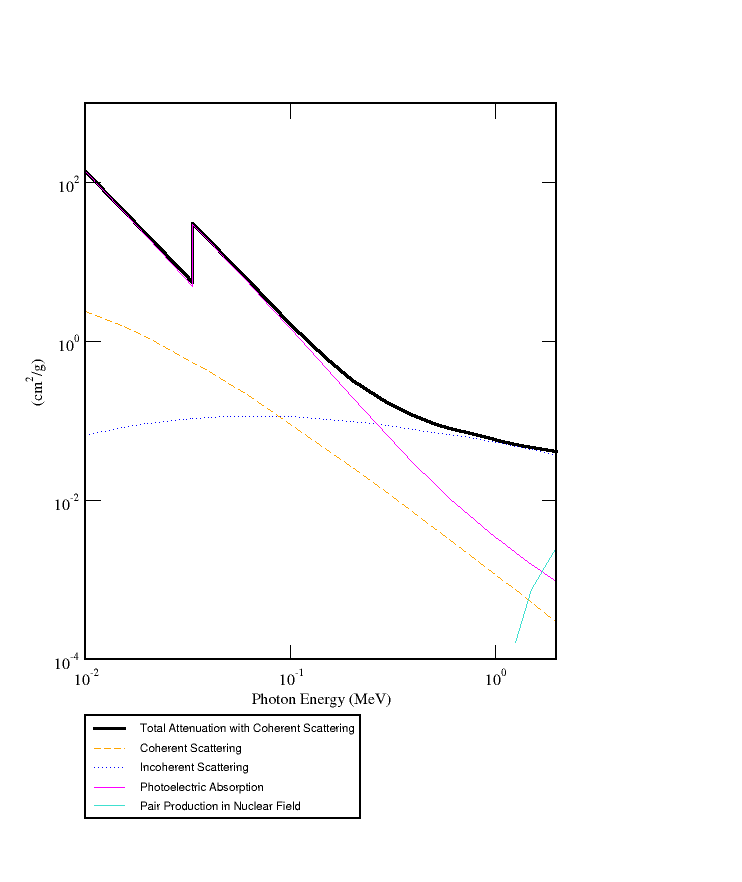
\includegraphics[width=28em]{photon_cross_section_xcom}
 	\caption{\label{fig:photon_cross_section_xcom}Sezione d'urto in funzione dell'energia per i vari processi nel NaI (densità $\rho = \SI{3.67}{g\;cm^3}$) FONTE CIPPALIAPPA}
 \end{figure}
 
 %%%%%%%%%%%%%%%%%%%%%%%%%%%%%%%%%%%%%%%%%%%%%%%%%%%%%%%%%%%%%%%%%%%%%%%%
 \subsubsection{Risposta attesa del detector}
 \paragraph{Grande detector} Se il detector fosse abbastanza esteso, tutta l'energia dei fotoni, indipendentemente dalla complessità dell'interazione, verrebbe rilasciata nel rivelatore. Per una sorgente di fotoni ad una energia fissata, come potrebbe essere una sorgente di raggi $\gamma$\footnote{I raggi $\gamma$ delle sorgenti radioattive hanno tipicamente larghezze $\Gamma \ll \SI{1}{eV}$ e possono quindi considerarsi mono-energetici per i nostri scopi.}, ad esempio il \cs, lo spettro energetico prodotto da un tale scintillatore sarebbe un singolo fotopicco all'energia dei fotoni $\gamma$ (vedi \autoref{fig.spettrometro_grosso} con una larghezza dovuta essenzialmente alla risoluzione dello strumento, come analizzeremo nel seguito.
 
 \begin{figure}[h]
 	\centering
 	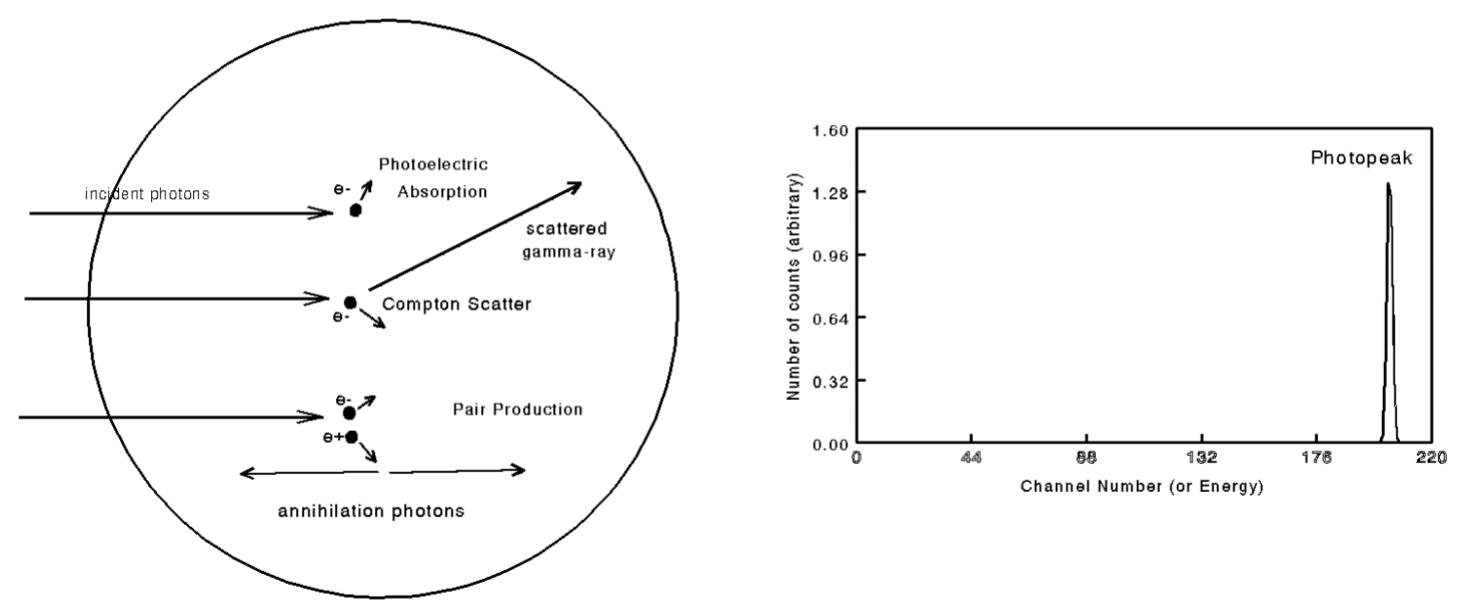
\includegraphics[width=28em]{spettrometro_grosso}
 	\caption{\label{fig:spettrometro_grsso}Risposta di un detector di grandi dimensioni per fotoni mono-energetici}
 \end{figure}

 \paragraph{Piccolo detector}Nel caso opposto di un detector di piccole dimensioni i fotoni potranno interagire una sola volta, facendo effetto fotoelettrico o Compton\footnote{Stiamo trascurando la produzione di coppie, per i motivi detti sopra} in proporzione alla sezione d'urto. I fotoni che fanno effetto fotoelettrico produrranno un segnale alla loro energia (che non sarà una delta ma sarà allargato dalla risoluzione strumentale) come visto prima, mentre i fotoni che faranno fotoelettrico si produrranno uno spettro come quello predetto dalla sezione d'urto di Klein-Nishina (la spalla Compton sarà meno definita perché convoluta con la risoluzione strumentale). Il risultato finale sarà simile a quelli in \autoref{spettrometro_piccolo}
 
  \begin{figure}[h]
 	\centering
 	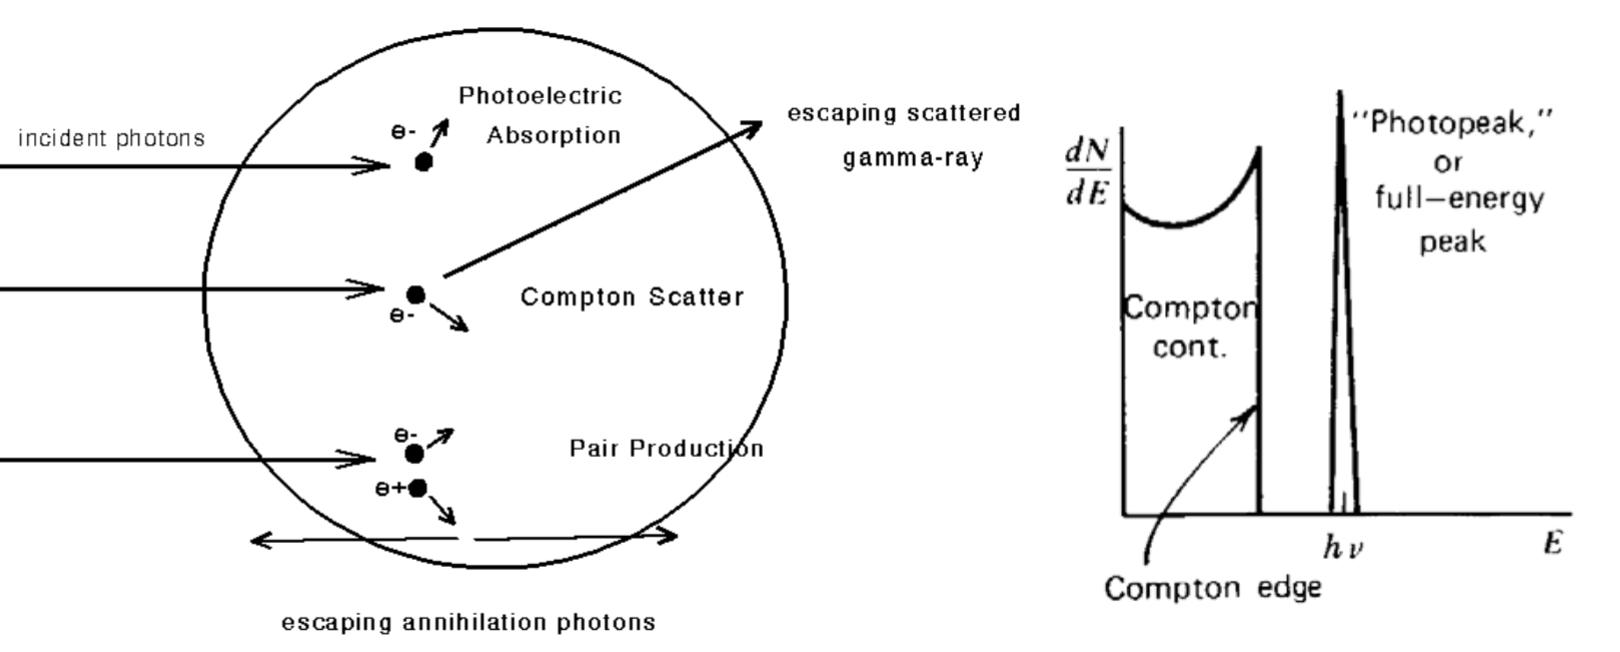
\includegraphics[width=28em]{spettrometro_piccolo}
 	\caption{\label{fig:spettrometro_piccolo}Risposta di un detector di piccole dimensioni per fotoni mono-energetici}
 \end{figure}
 
 \paragraph{Detector di dimensioni intermedie}Nel nostro caso disponiamo di un rivelatore $2"\times2"$ e, a partire dal grafico in FONTE che ci dà la lunghezza di radiazione al variare dell'energia del fotone in vari materiali, è semplice calcolare che per il nostro rivelatore la lunghezza di radiazione:$\sim \SI{5}{cm}$, quindi paragonabile alla dimensione del cristallo, ne segue che il $\sim 60\%$ dei fotoni interagisce nel cristallo almeno una volta. Ci troviamo quindi in una situazione intermedia per cui in pratica lo spettro sarà simile a quello in \autoref{spettrometro_piccolo}, ma il rapporto tra gli eventi Compton e quelli fotoelettrico non sarà uguale al rapporto tra le sezioni d'urto: è infatti importante il contributo di quei fotoni che dopo aver fatto Compton fanno fotoelettrico\footnote{Questa doppia interazione è anche favorita dal fatto che i fotoni che hanno fatto scattering Compton hanno perso energia e l'effetto fotoelettrico ha sezione d'urto maggiore al diminuire dell'energia} (quando ancora si trovano nello spettrometro): questi produrranno un segnale all'energia del fotopicco poiché tutta l'energia del fotone iniziale è rilasciata nello scintillatore. 
 
 Lo spettro finale prodotto sarà la somma di molti effetti riassunti in \autoref{spettrometro_intermedio}:
 \begin{itemize}
 	\item l'assorbimento fotoelettrico produrrà un fotopicco all'energia dei fotoni incidenti;
 	\item i fotoni che fanno scattering Compton rilasceranno solo parte della loro energia producendo il caratteristico profilo predetto dalla  formula di Klein-Nishina;
 	\item i fotoni che fanno scattering Compton sui materiali che circondano il detector possono tornare nello stesso producendo un picco, detto di backscattering nella regione a basse energie;
 	\item spesso potrebbe essere visibile un picco all'energia caratteristica dei raggi X emessi dai materiali circostanti (ad esempio lo stesso spettrometro);
 	\item se la soergente decade $\beta^+$ (come il \na) sarà visibile un fotopicco a \SI{511}keV dovuto ai fotoni $\gamma$ prodotti nell'annichilazione del positrone con la materia circostante.
 \end{itemize}
Lo spettro finale atteso (per una sorgente che emetta un solo fotone e uno spettrometro di dimensioni intermedie) è schematizzato in \autoref{fig:spettrometro_intermedio} e si può confrontare con un tipico spettro acquisito con il nostro spettrometro in \autoref{spettro_tipico} (si tratta del \cs\; che emette un fotone a \SI{662}keV)

 \begin{figure}[h]
	\centering
	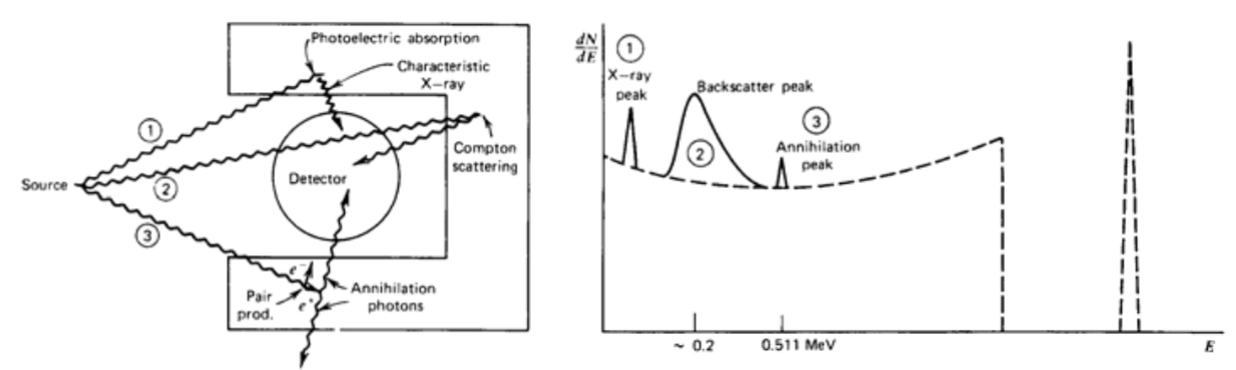
\includegraphics[width=28em]{spettrometro_intermedio}
	\caption{\label{fig:spettrometro_intermedio}Risposta di un detector di dimensioni intermedie (come il nostro) per fotoni mono-energetici}
 \end{figure}

 %%%%%%%%%%%%%%%%%%%%%%%%%%%%%%%%%%%%%%%%%%%%%%%%%%%%%%%%%%%%%%%%%%%%%%%%%%%%%%%%
 \subsubsection{Risposta del detector}
 
 \paragraph{Efficienza}
 
 \paragraph{Funzione di risposta (linearità)}
 Un rivelatore di radiazione ideale dovrebbe essere perfettamente lineare 
 
 \paragraph{Distribuzione di risposta (risoluzione)}
 
 
 
 
 
 